\begin{appendices}

%%%%%%%%%%%%%%%%%%%%%%%%%%%%%%%%%%%%%%%%%%%%%%%%%%%%%%%%%%%%%%%%%%%%%%%%%%%%%%%%%%

%\section{Selecting object categories}
%\label{sec:AppClasses}

\section{ILSVRC2012-2014 image classification and single-object localization object categories}
\label{app:classes}

{\tiny
%{\bf Image classification and single-object localization (1000 categories)}:
abacus, abaya, academic gown, accordion, acorn, acorn squash, acoustic guitar, admiral, affenpinscher, Afghan hound, African chameleon, African crocodile, African elephant, African grey, African hunting dog, agama, agaric, aircraft carrier, Airedale, airliner, airship, albatross, alligator lizard, alp, altar, ambulance, American alligator, American black bear, American chameleon, American coot, American egret, American lobster, American Staffordshire terrier, amphibian, analog clock, anemone fish, Angora, ant, apiary, Appenzeller, apron, Arabian camel, Arctic fox, armadillo, artichoke, ashcan, assault rifle, Australian terrier, axolotl, baboon, backpack, badger, bagel, bakery, balance beam, bald eagle, balloon, ballplayer, ballpoint, banana, Band Aid, banded gecko, banjo, bannister, barbell, barber chair, barbershop, barn, barn spider, barometer, barracouta, barrel, barrow, baseball, basenji, basketball, basset, bassinet, bassoon, bath towel, bathing cap, bathtub, beach wagon, beacon, beagle, beaker, bearskin, beaver, Bedlington terrier, bee, bee eater, beer bottle, beer glass, bell cote, bell pepper, Bernese mountain dog, bib, bicycle-built-for-two, bighorn, bikini, binder, binoculars, birdhouse, bison, bittern, black and gold garden spider, black grouse, black stork, black swan, black widow, black-and-tan coonhound, black-footed ferret, Blenheim spaniel, bloodhound, bluetick, boa constrictor, boathouse, bobsled, bolete, bolo tie, bonnet, book jacket, bookcase, bookshop, Border collie, Border terrier, borzoi, Boston bull, bottlecap, Bouvier des Flandres, bow, bow tie, box turtle, boxer, Brabancon griffon, brain coral, brambling, brass, brassiere, breakwater, breastplate, briard, Brittany spaniel, broccoli, broom, brown bear, bubble, bucket, buckeye, buckle, bulbul, bull mastiff, bullet train, bulletproof vest, bullfrog, burrito, bustard, butcher shop, butternut squash, cab, cabbage butterfly, cairn, caldron, can opener, candle, cannon, canoe, capuchin, car mirror, car wheel, carbonara, Cardigan, cardigan, cardoon, carousel, carpenter's kit, carton, cash machine, cassette, cassette player, castle, catamaran, cauliflower, CD player, cello, cellular telephone, centipede, chain, chain mail, chain saw, chainlink fence, chambered nautilus, cheeseburger, cheetah, Chesapeake Bay retriever, chest, chickadee, chiffonier, Chihuahua, chime, chimpanzee, china cabinet, chiton, chocolate sauce, chow, Christmas stocking, church, cicada, cinema, cleaver, cliff, cliff dwelling, cloak, clog, clumber, cock, cocker spaniel, cockroach, cocktail shaker, coffee mug, coffeepot, coho, coil, collie, colobus, combination lock, comic book, common iguana, common newt, computer keyboard, conch, confectionery, consomme, container ship, convertible, coral fungus, coral reef, corkscrew, corn, cornet, coucal, cougar, cowboy boot, cowboy hat, coyote, cradle, crane, crane, crash helmet, crate, crayfish, crib, cricket, Crock Pot, croquet ball, crossword puzzle, crutch, cucumber, cuirass, cup, curly-coated retriever, custard apple, daisy, dalmatian, dam, damselfly, Dandie Dinmont, desk, desktop computer, dhole, dial telephone, diamondback, diaper, digital clock, digital watch, dingo, dining table, dishrag, dishwasher, disk brake, Doberman, dock, dogsled, dome, doormat, dough, dowitcher, dragonfly, drake, drilling platform, drum, drumstick, dugong, dumbbell, dung beetle, Dungeness crab, Dutch oven, ear, earthstar, echidna, eel, eft, eggnog, Egyptian cat, electric fan, electric guitar, electric locomotive, electric ray, English foxhound, English setter, English springer, entertainment center, EntleBucher, envelope, Eskimo dog, espresso, espresso maker, European fire salamander, European gallinule, face powder, feather boa, fiddler crab, fig, file, fire engine, fire screen, fireboat, flagpole, flamingo, flat-coated retriever, flatworm, flute, fly, folding chair, football helmet, forklift, fountain, fountain pen, four-poster, fox squirrel, freight car, French bulldog, French horn, French loaf, frilled lizard, frying pan, fur coat, gar, garbage truck, garden spider, garter snake, gas pump, gasmask, gazelle, German shepherd, German short-haired pointer, geyser, giant panda, giant schnauzer, gibbon, Gila monster, go-kart, goblet, golden retriever, goldfinch, goldfish, golf ball, golfcart, gondola, gong, goose, Gordon setter, gorilla, gown, grand piano, Granny Smith, grasshopper, Great Dane, great grey owl, Great Pyrenees, great white shark, Greater Swiss Mountain dog, green lizard, green mamba, green snake, greenhouse, grey fox, grey whale, grille, grocery store, groenendael, groom, ground beetle, guacamole, guenon, guillotine, guinea pig, gyromitra, hair slide, hair spray, half track, hammer, hammerhead, hamper, hamster, hand blower, hand-held computer, handkerchief, hard disc, hare, harmonica, harp, hartebeest, harvester, harvestman, hatchet, hay, head cabbage, hen, hen-of-the-woods, hermit crab, hip, hippopotamus, hog, hognose snake, holster, home theater, honeycomb, hook, hoopskirt, horizontal bar, hornbill, horned viper, horse cart, hot pot, hotdog, hourglass, house finch, howler monkey, hummingbird, hyena, ibex, Ibizan hound, ice bear, ice cream, ice lolly, impala, Indian cobra, Indian elephant, indigo bunting, indri, iPod, Irish setter, Irish terrier, Irish water spaniel, Irish wolfhound, iron, isopod, Italian greyhound, jacamar, jack-o'-lantern, jackfruit, jaguar, Japanese spaniel, jay, jean, jeep, jellyfish, jersey, jigsaw puzzle, jinrikisha, joystick, junco, keeshond, kelpie, Kerry blue terrier, killer whale, kimono, king crab, king penguin, king snake, kit fox, kite, knee pad, knot, koala, Komodo dragon, komondor, kuvasz, lab coat, Labrador retriever, lacewing, ladle, ladybug, Lakeland terrier, lakeside, lampshade, langur, laptop, lawn mower, leaf beetle, leafhopper, leatherback turtle, lemon, lens cap, Leonberg, leopard, lesser panda, letter opener, Lhasa, library, lifeboat, lighter, limousine, limpkin, liner, lion, lionfish, lipstick, little blue heron, llama, Loafer, loggerhead, long-horned beetle, lorikeet, lotion, loudspeaker, loupe, lumbermill, lycaenid, lynx, macaque, macaw, Madagascar cat, magnetic compass, magpie, mailbag, mailbox, maillot, maillot, malamute, malinois, Maltese dog, manhole cover, mantis, maraca, marimba, marmoset, marmot, mashed potato, mask, matchstick, maypole, maze, measuring cup, meat loaf, medicine chest, meerkat, megalith, menu, Mexican hairless, microphone, microwave, military uniform, milk can, miniature pinscher, miniature poodle, miniature schnauzer, minibus, miniskirt, minivan, mink, missile, mitten, mixing bowl, mobile home, Model T, modem, monarch, monastery, mongoose, monitor, moped, mortar, mortarboard, mosque, mosquito net, motor scooter, mountain bike, mountain tent, mouse, mousetrap, moving van, mud turtle, mushroom, muzzle, nail, neck brace, necklace, nematode, Newfoundland, night snake, nipple, Norfolk terrier, Norwegian elkhound, Norwich terrier, notebook, obelisk, oboe, ocarina, odometer, oil filter, Old English sheepdog, orange, orangutan, organ, oscilloscope, ostrich, otter, otterhound, overskirt, ox, oxcart, oxygen mask, oystercatcher, packet, paddle, paddlewheel, padlock, paintbrush, pajama, palace, panpipe, paper towel, papillon, parachute, parallel bars, park bench, parking meter, partridge, passenger car, patas, patio, pay-phone, peacock, pedestal, Pekinese, pelican, Pembroke, pencil box, pencil sharpener, perfume, Persian cat, Petri dish, photocopier, pick, pickelhaube, picket fence, pickup, pier, piggy bank, pill bottle, pillow, pineapple, ping-pong ball, pinwheel, pirate, pitcher, pizza, plane, planetarium, plastic bag, plate, plate rack, platypus, plow, plunger, Polaroid camera, pole, polecat, police van, pomegranate, Pomeranian, poncho, pool table, pop bottle, porcupine, pot, potpie, potter's wheel, power drill, prairie chicken, prayer rug, pretzel, printer, prison, proboscis monkey, projectile, projector, promontory, ptarmigan, puck, puffer, pug, punching bag, purse, quail, quill, quilt, racer, racket, radiator, radio, radio telescope, rain barrel, ram, rapeseed, recreational vehicle, red fox, red wine, red wolf, red-backed sandpiper, red-breasted merganser, redbone, redshank, reel, reflex camera, refrigerator, remote control, restaurant, revolver, rhinoceros beetle, Rhodesian ridgeback, rifle, ringlet, ringneck snake, robin, rock beauty, rock crab, rock python, rocking chair, rotisserie, Rottweiler, rubber eraser, ruddy turnstone, ruffed grouse, rugby ball, rule, running shoe, safe, safety pin, Saint Bernard, saltshaker, Saluki, Samoyed, sandal, sandbar, sarong, sax, scabbard, scale, schipperke, school bus, schooner, scoreboard, scorpion, Scotch terrier, Scottish deerhound, screen, screw, screwdriver, scuba diver, sea anemone, sea cucumber, sea lion, sea slug, sea snake, sea urchin, Sealyham terrier, seashore, seat belt, sewing machine, Shetland sheepdog, shield, Shih-Tzu, shoe shop, shoji, shopping basket, shopping cart, shovel, shower cap, shower curtain, siamang, Siamese cat, Siberian husky, sidewinder, silky terrier, ski, ski mask, skunk, sleeping bag, slide rule, sliding door, slot, sloth bear, slug, snail, snorkel, snow leopard, snowmobile, snowplow, soap dispenser, soccer ball, sock, soft-coated wheaten terrier, solar dish, sombrero, sorrel, soup bowl, space bar, space heater, space shuttle, spaghetti squash, spatula, speedboat, spider monkey, spider web, spindle, spiny lobster, spoonbill, sports car, spotlight, spotted salamander, squirrel monkey, Staffordshire bullterrier, stage, standard poodle, standard schnauzer, starfish, steam locomotive, steel arch bridge, steel drum, stethoscope, stingray, stinkhorn, stole, stone wall, stopwatch, stove, strainer, strawberry, street sign, streetcar, stretcher, studio couch, stupa, sturgeon, submarine, suit, sulphur butterfly, sulphur-crested cockatoo, sundial, sunglass, sunglasses, sunscreen, suspension bridge, Sussex spaniel, swab, sweatshirt, swimming trunks, swing, switch, syringe, tabby, table lamp, tailed frog, tank, tape player, tarantula, teapot, teddy, television, tench, tennis ball, terrapin, thatch, theater curtain, thimble, three-toed sloth, thresher, throne, thunder snake, Tibetan mastiff, Tibetan terrier, tick, tiger, tiger beetle, tiger cat, tiger shark, tile roof, timber wolf, titi, toaster, tobacco shop, toilet seat, toilet tissue, torch, totem pole, toucan, tow truck, toy poodle, toy terrier, toyshop, tractor, traffic light, trailer truck, tray, tree frog, trench coat, triceratops, tricycle, trifle, trilobite, trimaran, tripod, triumphal arch, trolleybus, trombone, tub, turnstile, tusker, typewriter keyboard, umbrella, unicycle, upright, vacuum, valley, vase, vault, velvet, vending machine, vestment, viaduct, vine snake, violin, vizsla, volcano, volleyball, vulture, waffle iron, Walker hound, walking stick, wall clock, wallaby, wallet, wardrobe, warplane, warthog, washbasin, washer, water bottle, water buffalo, water jug, water ouzel, water snake, water tower, weasel, web site, weevil, Weimaraner, Welsh springer spaniel, West Highland white terrier, whippet, whiptail, whiskey jug, whistle, white stork, white wolf, wig, wild boar, window screen, window shade, Windsor tie, wine bottle, wing, wire-haired fox terrier, wok, wolf spider, wombat, wood rabbit, wooden spoon, wool, worm fence, wreck, yawl, yellow lady's slipper, Yorkshire terrier, yurt, zebra, zucchini

}

%\noindent
%{\bf Object detection (200 categories)}:
%\input{det_hierarchy.tex}
%}


%%%%%%%%%%%%%%%%%%%%%%%%%%%%%%%%%%%%%%%%%%%%%%%%%%%%%%%%%%%%%%%%%%%%%%%%%%%%%%%%%%

\section{Additional single-object localization dataset statistics}
\label{app:ICCV}

We consider two additional metrics of object localization difficulty: chance performance of localization and the level of clutter. We use these metrics to compare ILSVRC2012-2014
single-object localization dataset to the PASCAL VOC 2012 object detection benchmark. The measures of localization difficulty are computed on the validation set of both datasets. According to both of these measures of difficulty there is a subset of ILSVRC which is as challenging as PASCAL but more than an order of magnitude greater in size. Figure~\ref{fig:locdiff} shows the distributions of different properties (object scale, chance performance of localization and level of clutter) across the different classes in the two datasets.

\iffalse
\begin{table}
{\small
\begin{tabular}{|c|c|c|c|}
\hline
Property & PASCAL & ILSVRC subset & ILSVRC \\
%\hline
%SCALE & 24.08\%  & 24.06\% (537) & 35.83\% \\
\hline
Instances & 1.69 (20) & 1.69 (843)  & 1.61 (1000)\\
\hline
%Neighbors & 0.52 (20) & 0.52 (913) & 0.47 (1000)\\
%\hline
CPL & 8.76\%  (20) & 8.74\% (562) & 20.83\% (1000) \\
\hline
Clutter & 5.90  (20) & 5.90 (250) & 3.59 (1000)\\
\hline
\end{tabular}
}
\caption{Comparison of the PASCAL VOC 2012 object detection dataset and the ILSVRC 2012 single-object localization dataset on several key properties of object localization difficulty (please see Section~\ref{sec:LocStats} for definitions). For each property, the ILSVRC subset is chosen by selecting the largest set of ILSVRC classes with the same average difficulty as that of the PASCAL classes. The number of object classes is indicated in parentheses.  Note that according to any of these measures of difficulty there is a subset of ILSVRC which is as challenging as PASCAL but more than an order of magnitude greater in size.}
\label{table:impascal}
\end{table}
\fi



\paragraph{Chance performance of localization (CPL).} Chance performance on a dataset is a common metric to consider. We define the CPL measure as the expected accuracy of a detector which first randomly samples an object instance of that class and then uses its bounding box directly as the proposed localization window on all other images (after rescaling the images to the same size). Concretely, let $B_1,B_2,\dots,B_N$ be all the bounding boxes of the object instances within a class, then
\begin{equation}
\label{cpleq}
\mbox{\sc CPL} = \frac{\sum_i \sum_{j \neq i} IOU(B_i,B_j)\geq 0.5}{N(N-1)}
\end{equation}
Some of the most difficult ILSVRC categories to localize according to this metric are basketball, swimming trunks, ping pong ball and rubber eraser, all with less than $0.2\%$ CPL. This measure correlates strongly ($\rho = 0.9$) with the average scale of the object (fraction of image occupied by object). The average CPL across the $1000$ ILSVRC categories is $20.8\%$. The 20 PASCAL categories have an average CPL of $8.7\%$, which is the same as the CPL of the $562$ most difficult categories of ILSVRC.

\paragraph{Clutter.} Intuitively, even small objects are easy to localize on a plain background. To quantify clutter we employ the objectness measure of~\citep{Alexe12}, which is a class-generic object detector evaluating how likely a window in the image contains a coherent object (of any class) as opposed to background (sky, water, grass). For every image $m$ containing target object instances at positions $B_1^m,B_2^m,\dots$, we use the publicly available objectness software to sample 1000 windows $W_1^m,W_2^m,\dots W_{1000}^m$, in order of decreasing probability of the window containing any generic object. Let {\sc obj}(m) be the number of generic object-looking windows sampled before localizing an instance of the target category, i.e., $\mbox{\sc obj}(m) = \min \{k: \max_i \mbox{\sc iou}(W_k^m,B_i^m) \geq 0.5\}$. For a category containing M images, we compute the average number of such windows per image and define
\begin{equation}
\label{cluttereq}
\textstyle
\mbox{\sc Clutter} = \log_{2} \large ( \frac{1}{M}\sum_m \mbox{\sc obj}(m) \large )
\end{equation}
The higher the clutter of a category, the harder the objects are to localize according to generic cues. If an object can't be localized with the first 1000 windows (as is the case for $1\%$ of images on average per category in ILSVRC and $5\%$ in PASCAL), we set {\sc obj}$(m)=1001$. The fact that more than $95\%$ of objects can be localized with these windows imply that the objectness cue is already quite strong, so objects that require many windows on average will be extremely difficult to detect: e.g., ping pong ball (clutter of 9.57, or 758 windows on average), basketball (clutter of 9.21), puck (clutter of 9.17) in ILSVRC. The most difficult object in PASCAL is bottle with clutter score of $8.47$.  On average, ILSVRC has clutter score of $3.59$. The most difficult subset of ILSVRC with 250 object categories has an order of magnitude more categories and the same average amount of clutter (of $5.90$) as the PASCAL dataset. 

\begin{figure*}
\center{{\bf 1000 classes of ILSVRC2012-2014 single-object localization (dark green) \\ versus 20 classes of PASCAL 2012 (light blue)}}
\begin{tabular}{p{0.22\textwidth} p{0.22\textwidth} p{0.22\textwidth} p{0.22\textwidth}}
\center{$\rightarrow$ more diffiult} & 
\center{more diffiult $\leftarrow$}  &
\center{more diffiult $\leftarrow$}  &
\center{ $\rightarrow$ more diffiult}
\end{tabular}
\\
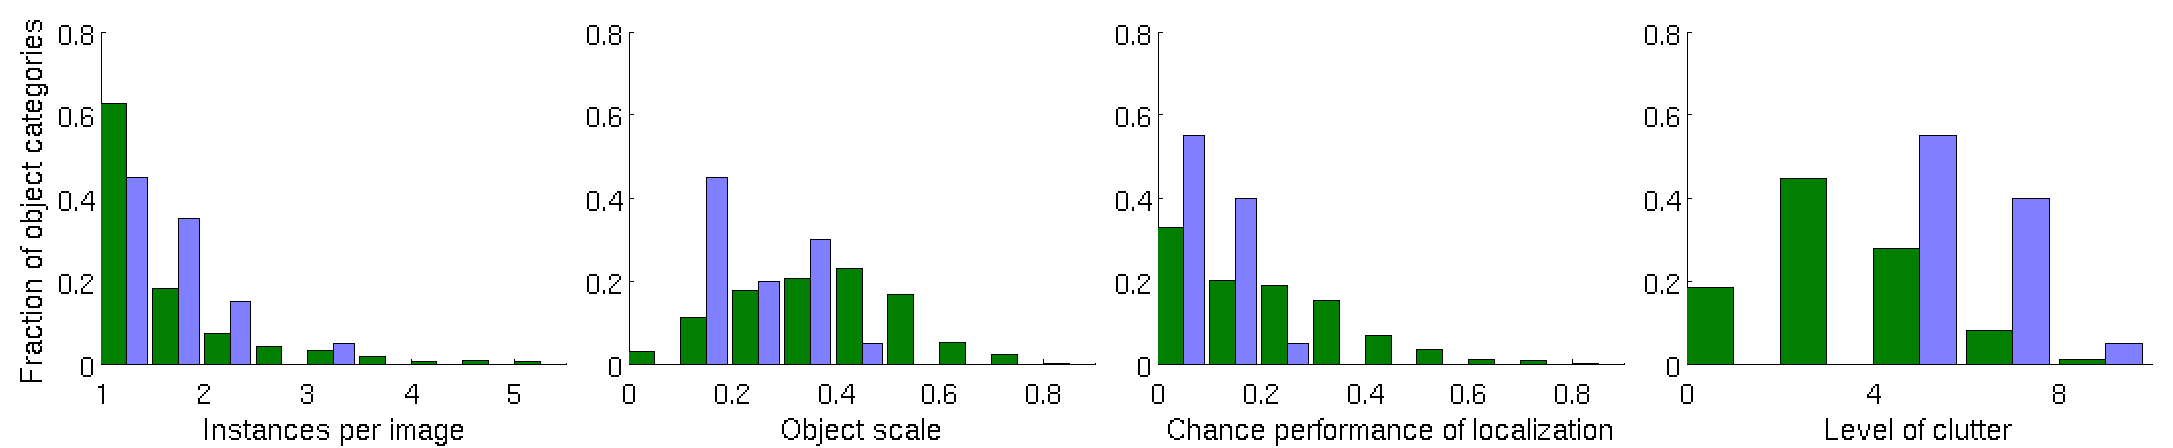
\includegraphics[width=\textwidth]{clsloc_hist_supp.png} \\
\center{{\bf 200 hardest classes of ILSVRC2012-2014 single-object localization (dark green) \\ versus 20 classes of PASCAL 2012  (light blue)}}
\begin{tabular}{p{0.22\textwidth} p{0.22\textwidth} p{0.22\textwidth} p{0.22\textwidth}}
\center{$\rightarrow$ more diffiult} & 
\center{more diffiult $\leftarrow$}  &
\center{more diffiult $\leftarrow$}  &
\center{ $\rightarrow$ more diffiult}
\end{tabular}
\\
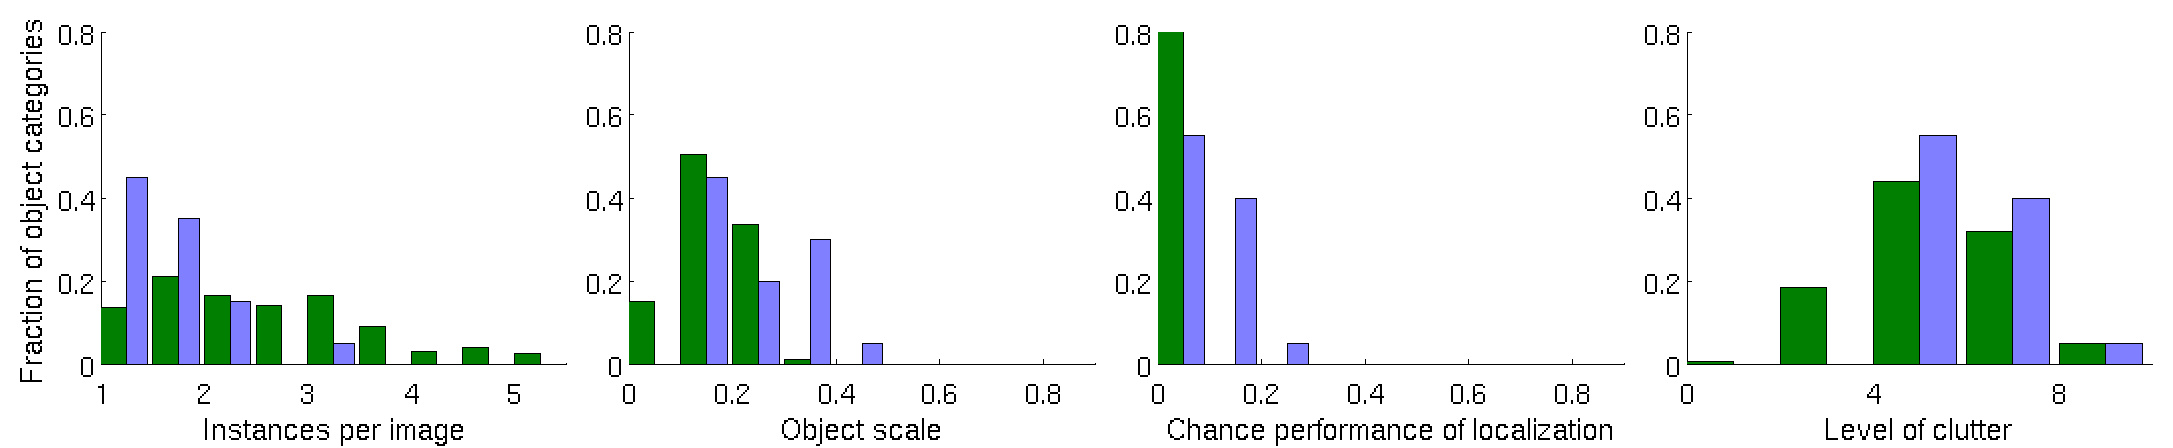
\includegraphics[width=\textwidth]{clsloc_hist_norm_supp.png} \\
\caption{Distribution of various measures of localization difficulty on the ILSVRC2012-2014 single-object localization (dark green) and PASCAL VOC 2012 (light blue) validation sets. Object scale is fraction of image area occupied by an average object instance. Chance performance of localization and level of clutter are defined in Appendix~\ref{app:ICCV}. The plots on top contain the full ILSVRC validation set with 1000 classes; the plots on the bottom contain 200 ILSVRC classes with the lowest chance performance of localization. All plots contain all 20 classes of PASCAL VOC. 
}
\label{fig:locdiff}
\end{figure*}



%%%%%%%%%%%%%%%%%%%%%%%%%%%%%%%%%%%%%%%%%%%%%%%%%%%%%%%%%%%%%%%%%%%%%%%%%%%%%%%%%%

\iffalse

%\section{Complete image-object annotation}
%\label{sec:AppChi}



With this algorithm in mind, the hierarchy of questions was constructed following the principle that false positives only add extra cost whereas false
negatives can significantly affect the quality of the labeling. 
%Figure~\ref{fig:qhierarchy} shows the constructed hierarchy. 
This was a surprisingly time-consuming process, involving multiple iterations, to ensure high accuracy of labeling and avoid false negatives.
\fi
\iffalse
\begin{figure}

\caption{The constructed hierarchy of questions for complete multi-class annotation.}
\label{fig:qhierarchy}
\end{figure}
\fi

\section{Manually curated queries for obtaining object detection scene images}
\label{sec:AppQueries}

In Section~\ref{sec:AnnotDetImages} we discussed three types of queries we used for collecting the object detection images:
(1) single object category name or a synonym; (2) a pair of object category names; (3) a manual query, typically targetting one or more object categories with insufficient data.
Here we provide a list of the 129 manually curated queries:

\vspace{0.1in}

{\tiny

\noindent 
afternoon tea, ant bridge building, armadillo race, armadillo yard, artist studio, auscultation, baby room, banjo orchestra, banjo rehersal, banjo show, califone headphones \& media player sets, camel dessert, camel tourist, carpenter drilling, carpentry, centipede wild, coffee shop, continental breakfast toaster, continental breakfast waffles, crutch walking, desert scorpion, diner, dining room, dining table, dinner, dragonfly friendly, dragonfly kid, dragonfly pond, dragonfly wild, drying hair, dumbbell curl, fan blow wind, fast food, fast food restaurant, firewood chopping, flu shot, goldfish aquarium, goldfish tank, golf cart on golf course, gym dumbbell, hamster drinking water, harmonica orchestra, harmonica rehersal, harmonica show, harp ensemble, harp orchestra, harp rehersal, harp show, hedgehog cute, hedgehog floor, hedgehog hidden, hippo bird, hippo friendly, home improvement diy drill, horseback riding, hotel coffee machine, hotel coffee maker, hotel waffle maker, jellyfish scuba, jellyfish snorkling, kitchen, kitchen counter coffee maker, kitchen counter toaster, kitchenette, koala feed, koala tree, ladybug flower, ladybug yard, laundromat, lion zebra friendly, lunch, mailman, making breakfast, making waffles, mexican food, motorcycle racing, office, office fan, opossum on tree branch, orchestra, panda play, panda tree, pizzeria, pomegranate tree, porcupine climbing trees, power drill carpenter, purse shop, red panda tree, riding competition, riding motor scooters, school supplies, scuba starfish, sea lion beach, sea otter, sea urchin habitat, shopping for school supplies, sitting in front of a fan, skunk and cat, skunk park, skunk wild, skunk yard, snail flower, snorkling starfish, snowplow cleanup, snowplow pile, snowplow winter, soccer game, south american zoo, starfish sea world, starts shopping, steamed artichoke, stethoscope doctor, strainer pasta, strainer tea, syringe doctor, table with food, tape player, tiger circus, tiger pet, using a can opener, using power drill, waffle iron breakfast, wild lion savana, wildlife preserve animals, wiping dishes, wombat petting zoo, zebra savana, zoo feeding, zoo in australia

}

%%%%%%%%%%%%%%%%%%%%%%%%%%%%%%%%%%%%
%\section{Comparison of ILSVRC object detection dataset with PASCAL VOC}

\iffalse
\begin{table}[t]
\centering
\begin{tabular}{|l|l|}
\hline
{\bf PASCAL VOC} & {\bf Closest ILSVRC-DET class} \\
{\bf (20 classes)} & {\bf (200 classes total)} \\
%{\bf PASCAL VOC (20) } & {\bf Closest ILSVRC-DET (200)} \\
%PASCAL VOC class & Closest of ILSVRC-DET classes \\
\hline
aeroplane & airplane\\
\hline
bicycle & bicycle \\
\hline
bird & bird \\
\hline
\emph{boat} & \emph{watercraft} \\
\hline
\emph{bottle} & \emph{wine bottle (or water bottle)}\\
\hline
bus & bus \\
\hline
car & car \\
\hline
cat & domestic cat \\
\hline
chair & chair \\
\hline
\emph{cow} & \emph{cattle} \\
\hline
\emph{dining table} & \emph{table} \\
\hline
dog & dog \\
\hline
horse & horse \\
\hline
motorbike & motorcyle \\
\hline
person & person \\
\hline
\emph{potted plant} & \emph{flower pot}\\
\hline
sheep & sheep \\
\hline
sofa & sofa \\
\hline
train & train \\
\hline
tv/monitor & tv or monitor \\
\hline
\end{tabular}
\caption{Correspondences between the object classes in the PASCAL VOC and the ILSVRC detection task.}
\label{table:detclassespascal}
\end{table}
\fi

\iffalse
\begin{table*}[t]
\centering
\begin{tabular}{|l |l |c|c|c|c|}
\hline
{\bf PASCAL VOC} & {\bf Closest ILSVRC-DET class} 
& \multicolumn{2}{c|}{Average object scale} 
& \multicolumn{2}{c|}{RCNN AP}  \\
\cline{3-6}
(20 classes) & (200 classes total) & PASCAL & ILSVRC & PASCAL & ILSVRC 
\\
%{\bf PASCAL VOC (20) } & {\bf Closest ILSVRC-DET (200)} \\
%PASCAL VOC class & Closest of ILSVRC-DET classes \\
\hline
aeroplane & airplane & 0.28 & 0.47\\
\hline
bicycle & bicycle & 0.29 & 0.46 \\
\hline
bird & bird \\
\hline
\emph{boat} & \emph{watercraft} \\
\hline
\emph{bottle} & \emph{wine bottle (or water bottle)}\\
\hline
bus & bus \\
\hline
car & car \\
\hline
cat & domestic cat \\
\hline
chair & chair \\
\hline
\emph{cow} & \emph{cattle} \\
\hline
\emph{dining table} & \emph{table} \\
\hline
dog & dog \\
\hline
horse & horse \\
\hline
motorbike & motorcyle \\
\hline
person & person \\
\hline
\emph{potted plant} & \emph{flower pot}\\
\hline
sheep & sheep \\
\hline
sofa & sofa \\
\hline
train & train \\
\hline
tv/monitor & tv or monitor \\
\hline
\end{tabular}
\caption{Correspondences between the object classes in the PASCAL VOC and the ILSVRC detection task.}
\label{table:detclassespascal}
\end{table*}

\fi


%%%%%%%%%%%%%%%%%%%%%%%%%%%%%%%%%%%%%%%%%%%%%%%%%%%%%%%%%%%%%%%%%%%%%%%%%%%%%%%%%%

\section{Hierarchy of questions for full image annotation}
\label{app:hierarchy}

The following is a hierarchy of questions manually constructed for crowdsourcing full annotation of images with the presence or absence of 200 object detection categories in ILSVRC2013 and ILSVRC2014. 
All questions are of the form ``is there a ... in the image?'' Questions marked with $\bullet$ are asked on every image.  If the answer to a question is determined to be ``no'' then the answer to all descendant questions is assumed to be ``no''. The 200 numbered leaf nodes correspond to the 200 object detection categories. 

The goal in the hierarchy construction is to save cost (by asking as few questions as possible on every image) while avoiding any ambiguity
in questions which would lead to false negatives during annotation. This hierarchy is not tree-structured; some questions have multiple parents. 

\vspace{0.1in}

{\tiny
\noindent {\bf Hierarchy of questions:} \\
\noindent \leftskip=0.0cm $\bullet$ first aid/ medical items

\noindent \leftskip=0.25cm $\circ$ (1) stethoscope

\noindent \leftskip=0.25cm $\circ$ (2) syringe

\noindent \leftskip=0.25cm $\circ$ (3) neck brace

\noindent \leftskip=0.25cm $\circ$ (4) crutch

\noindent \leftskip=0.25cm $\circ$ (5) stretcher

\noindent \leftskip=0.25cm $\circ$ (6) band aid: an adhesive bandage to cover small cuts or blisters

\noindent \leftskip=0.0cm $\bullet$ musical instruments

\noindent \leftskip=0.25cm $\circ$ (7) accordion (a portable box-shaped free-reed instrument; the reeds are made to vibrate by air from the bellows controlled by the player)

\noindent \leftskip=0.25cm $\circ$ (8) piano, pianoforte, forte-piano

\noindent \leftskip=0.25cm $\circ$ percussion instruments: chimes, maraccas, drums, etc

\noindent \leftskip=0.5cm $\circ$ (9) chime: a percussion instrument consisting of a set of tuned bells that are struck with a hammer; used as an orchestral instrument

\noindent \leftskip=0.5cm $\circ$ (10) maraca

\noindent \leftskip=0.5cm $\circ$ (11) drum

\noindent \leftskip=0.25cm $\circ$ stringed instrument

\noindent \leftskip=0.5cm $\circ$ (12) banjo, the body of a banjo is round.  please do not confuse with guitar

\noindent \leftskip=0.5cm $\circ$ (13) cello: a large stringed instrument; seated player holds it upright while playing

\noindent \leftskip=0.5cm $\circ$ (14) violin: bowed stringed instrument that has four strings, a hollow body, an unfretted fingerboard and is played with a bow. please do not confuse with cello, which is held upright while playing

\noindent \leftskip=0.5cm $\circ$ (15) harp

\noindent \leftskip=0.5cm $\circ$ (16) guitar, please do not confuse with banjo.  the body of a banjo is round

\noindent \leftskip=0.25cm $\circ$ wind instrument: a musical instrument in which the sound is produced by an enclosed column of air that is moved by the breath (such as trumpet, french horn, harmonica, flute, etc)

\noindent \leftskip=0.5cm $\circ$ (17) trumpet: a brass musical instrument with a narrow tube and a flared bell, which is played by means of valves. often has 3 keys on top

\noindent \leftskip=0.5cm $\circ$ (18) french horn: a brass musical instrument consisting of a conical tube that is coiled into a spiral, with a flared bell at the end

\noindent \leftskip=0.5cm $\circ$ (19) trombone: a brass instrument consisting of a long tube whose length can be varied by a u-shaped slide

\noindent \leftskip=0.5cm $\circ$ (20) harmonica

\noindent \leftskip=0.5cm $\circ$ (21) flute: a high-pitched musical instrument that looks like a straight tube and is usually played sideways (please do not confuse with oboes, which have a distinctive straw-like mouth piece and a slightly flared end)

\noindent \leftskip=0.5cm $\circ$ (22) oboe: a slender musical instrument roughly 65cm long with metal keys, a distinctive straw-like mouthpiece and often a slightly flared end (please do not confuse with flutes)

\noindent \leftskip=0.5cm $\circ$ (23) saxophone: a musical instrument consisting of a brass conical tube, often with a u-bend at the end

\noindent \leftskip=0.0cm $\bullet$ food: something you can eat or drink (includes growing fruit, vegetables and mushrooms, but does not include living animals)

\noindent \leftskip=0.25cm $\circ$ food with bread or crust: pretzel, bagel, pizza, hotdog, hamburgers, etc

\noindent \leftskip=0.5cm $\circ$ (24) pretzel

\noindent \leftskip=0.5cm $\circ$ (25) bagel, beigel

\noindent \leftskip=0.5cm $\circ$ (26) pizza, pizza pie

\noindent \leftskip=0.5cm $\circ$ (27) hotdog, hot dog, red hot

\noindent \leftskip=0.5cm $\circ$ (28) hamburger, beefburger, burger

\noindent \leftskip=0.25cm $\circ$ (29) guacamole

\noindent \leftskip=0.25cm $\circ$ (30) burrito

\noindent \leftskip=0.25cm $\circ$ (31) popsicle (ice cream or water ice on a small wooden stick)

\noindent \leftskip=0.25cm $\circ$ fruit

\noindent \leftskip=0.5cm $\circ$ (32) fig

\noindent \leftskip=0.5cm $\circ$ (33) pineapple, ananas

\noindent \leftskip=0.5cm $\circ$ (34) banana

\noindent \leftskip=0.5cm $\circ$ (35) pomegranate

\noindent \leftskip=0.5cm $\circ$ (36) apple

\noindent \leftskip=0.5cm $\circ$ (37) strawberry

\noindent \leftskip=0.5cm $\circ$ (38) orange

\noindent \leftskip=0.5cm $\circ$ (39) lemon

\noindent \leftskip=0.25cm $\circ$ vegetables

\noindent \leftskip=0.5cm $\circ$ (40) cucumber, cuke

\noindent \leftskip=0.5cm $\circ$ (41) artichoke, globe artichoke

\noindent \leftskip=0.5cm $\circ$ (42) bell pepper

\noindent \leftskip=0.5cm $\circ$ (43) head cabbage

\noindent \leftskip=0.25cm $\circ$ (44) mushroom

\noindent \leftskip=0.0cm $\bullet$ items that run on electricity (plugged in or using batteries); including clocks, microphones, traffic lights, computers, etc

\noindent \leftskip=0.25cm $\circ$ (45) remote control, remote

\noindent \leftskip=0.25cm $\circ$ electronics that blow air

\noindent \leftskip=0.5cm $\circ$ (46) hair dryer, blow dryer

\noindent \leftskip=0.5cm $\circ$ (47) electric fan: a device for creating a current of air by movement of a surface or surfaces (please do not consider hair dryers)

\noindent \leftskip=0.25cm $\circ$ electronics that can play music or amplify sound

\noindent \leftskip=0.5cm $\circ$ (48) tape player

\noindent \leftskip=0.5cm $\circ$ (49) iPod

\noindent \leftskip=0.25cm $\circ$ (50) microphone, mike

\noindent \leftskip=0.25cm $\circ$ computer and computer peripherals: mouse, laptop, printer, keyboard, etc

\noindent \leftskip=0.5cm $\circ$ (51) computer mouse

\noindent \leftskip=0.5cm $\circ$ (52) laptop, laptop computer

\noindent \leftskip=0.5cm $\circ$ (53) printer (please do not consider typewriters to be printers)

\noindent \leftskip=0.5cm $\circ$ (54) computer keyboard

\noindent \leftskip=0.25cm $\circ$ (55) lamp

\noindent \leftskip=0.25cm $\circ$ electric cooking appliance (an appliance which generates heat to cook food or boil water)

\noindent \leftskip=0.5cm $\circ$ (56) microwave, microwave oven

\noindent \leftskip=0.5cm $\circ$ (57) toaster

\noindent \leftskip=0.5cm $\circ$ (58) waffle iron

\noindent \leftskip=0.5cm $\circ$ (59) coffee maker: a kitchen appliance used for brewing coffee automatically

\noindent \leftskip=0.25cm $\circ$ (60) vacuum, vacuum cleaner

\noindent \leftskip=0.25cm $\circ$ (61) dishwasher, dish washer, dishwashing machine

\noindent \leftskip=0.25cm $\circ$ (62) washer, washing machine: an electric appliance for washing clothes

\noindent \leftskip=0.25cm $\circ$ (63) traffic light, traffic signal, stoplight

\noindent \leftskip=0.25cm $\circ$ (64) tv or monitor: an electronic device that represents information in visual form

\noindent \leftskip=0.25cm $\circ$ (65) digital clock: a clock that displays the time of day digitally

\noindent \leftskip=0.0cm $\bullet$ kitchen items: tools,utensils and appliances usually found in the kitchen

\noindent \leftskip=0.25cm $\circ$ electric cooking appliance (an appliance which generates heat to cook food or boil water)

\noindent \leftskip=0.5cm $\circ$ (56) microwave, microwave oven

\noindent \leftskip=0.5cm $\circ$ (57) toaster

\noindent \leftskip=0.5cm $\circ$ (58) waffle iron

\noindent \leftskip=0.5cm $\circ$ (59) coffee maker: a kitchen appliance used for brewing coffee automatically

\noindent \leftskip=0.25cm $\circ$ (61) dishwasher, dish washer, dishwashing machine

\noindent \leftskip=0.25cm $\circ$ (66) stove

\noindent \leftskip=0.25cm $\circ$ things used to open cans/bottles: can opener or corkscrew

\noindent \leftskip=0.5cm $\circ$ (67) can opener (tin opener)

\noindent \leftskip=0.5cm $\circ$ (68) corkscrew

\noindent \leftskip=0.25cm $\circ$ (69) cocktail shaker

\noindent \leftskip=0.25cm $\circ$ non-electric item commonly found in the kitchen: pot, pan, utensil, bowl, etc

\noindent \leftskip=0.5cm $\circ$ (70) strainer

\noindent \leftskip=0.5cm $\circ$ (71) frying pan (skillet)

\noindent \leftskip=0.5cm $\circ$ (72) bowl: a dish for serving food that is round, open at the top, and has no handles (please do not confuse with a cup, which usually has a handle and is used for serving drinks)

\noindent \leftskip=0.5cm $\circ$ (73) salt or pepper shaker: a shaker with a perforated top for sprinkling salt or pepper

\noindent \leftskip=0.5cm $\circ$ (74) plate rack

\noindent \leftskip=0.5cm $\circ$ (75) spatula: a turner with a narrow flexible blade

\noindent \leftskip=0.5cm $\circ$ (76) ladle: a spoon-shaped vessel with a long handle; frequently used to transfer liquids from one container to another

\noindent \leftskip=0.25cm $\circ$ (77) refrigerator, icebox

\noindent \leftskip=0.0cm $\bullet$ furniture (including benches)

\noindent \leftskip=0.25cm $\circ$ (78) bookshelf:  a shelf on which to keep books

\noindent \leftskip=0.25cm $\circ$ (79) baby bed: small bed for babies, enclosed by sides to prevent baby from falling

\noindent \leftskip=0.25cm $\circ$ (80) filing cabinet: office furniture consisting of a container for keeping papers in order

\noindent \leftskip=0.25cm $\circ$ (81) bench (a long seat for several people, typically made of wood or stone)

\noindent \leftskip=0.25cm $\circ$ (82) chair: a raised piece of furniture for one person to sit on; please do not confuse with benches or sofas, which are made for more people

\noindent \leftskip=0.25cm $\circ$ (83) sofa, couch: upholstered seat for more than one person; please do not confuse with benches (which are made of wood or stone) or with chairs (which are for just one person)

\noindent \leftskip=0.25cm $\circ$ (84) table

\noindent \leftskip=0.0cm $\bullet$ clothing, article of clothing: a covering designed to be worn on a person's body

\noindent \leftskip=0.25cm $\circ$ (85) diaper: Garment consisting of a folded cloth drawn up between the legs and fastened at the waist; worn by infants to catch excrement

\noindent \leftskip=0.25cm $\circ$ swimming attire: clothes used for swimming or bathing (swim suits, swim trunks, bathing caps)

\noindent \leftskip=0.5cm $\circ$ (86) swimming trunks: swimsuit worn by men while swimming

\noindent \leftskip=0.5cm $\circ$ (87) bathing cap, swimming cap: a cap worn to keep hair dry while swimming or showering

\noindent \leftskip=0.5cm $\circ$ (88) maillot: a woman's one-piece bathing suit

\noindent \leftskip=0.25cm $\circ$ necktie: a man's formal article of clothing worn around the neck (including bow ties)

\noindent \leftskip=0.5cm $\circ$ (89) bow tie: a man's tie that ties in a bow

\noindent \leftskip=0.5cm $\circ$ (90) tie: a long piece of cloth worn for decorative purposes around the neck or shoulders, resting under the shirt collar and knotted at the throat (NOT a bow tie)

\noindent \leftskip=0.25cm $\circ$ headdress, headgear: clothing for the head (hats, helmets, bathing caps, etc)

\noindent \leftskip=0.5cm $\circ$ (87) bathing cap, swimming cap: a cap worn to keep hair dry while swimming or showering

\noindent \leftskip=0.5cm $\circ$ (91) hat with a wide brim

\noindent \leftskip=0.5cm $\circ$ (92) helmet: protective headgear made of hard material to resist blows

\noindent \leftskip=0.25cm $\circ$ (93) miniskirt, mini: a very short skirt

\noindent \leftskip=0.25cm $\circ$ (94) brassiere, bra: an undergarment worn by women to support their breasts

\noindent \leftskip=0.25cm $\circ$ (95) sunglasses

\noindent \leftskip=0.0cm $\bullet$ living organism (other than people): dogs, snakes, fish, insects, sea urchins, starfish, etc.

\noindent \leftskip=0.25cm $\circ$ living organism which can fly

\noindent \leftskip=0.5cm $\circ$ (96) bee

\noindent \leftskip=0.5cm $\circ$ (97) dragonfly

\noindent \leftskip=0.5cm $\circ$ (98) ladybug

\noindent \leftskip=0.5cm $\circ$ (99) butterfly

\noindent \leftskip=0.5cm $\circ$ (100) bird

\noindent \leftskip=0.25cm $\circ$ living organism which cannot fly (please don't include humans)

\noindent \leftskip=0.5cm $\circ$ living organism with 2 or 4 legs (please don't include humans):

\noindent \leftskip=0.75cm $\circ$ mammals (but please do not include humans)

\noindent \leftskip=1.0cm $\circ$ feline (cat-like) animal: cat, tiger or lion

\noindent \leftskip=1.25cm $\circ$ (101) domestic cat

\noindent \leftskip=1.25cm $\circ$ (102) tiger

\noindent \leftskip=1.25cm $\circ$ (103) lion

\noindent \leftskip=1.0cm $\circ$ canine (dog-like animal): dog, hyena, fox or wolf

\noindent \leftskip=1.25cm $\circ$ (104) dog, domestic dog, canis familiaris

\noindent \leftskip=1.25cm $\circ$ (105) fox: wild carnivorous mammal with pointed muzzle and ears and a bushy tail (please do not confuse with dogs)

\noindent \leftskip=1.0cm $\circ$ animals with hooves: camels, elephants, hippos, pigs, sheep, etc

\noindent \leftskip=1.25cm $\circ$ (106) elephant

\noindent \leftskip=1.25cm $\circ$ (107) hippopotamus, hippo

\noindent \leftskip=1.25cm $\circ$ (108) camel

\noindent \leftskip=1.25cm $\circ$ (109) swine: pig or boar

\noindent \leftskip=1.25cm $\circ$ (110) sheep: woolly animal, males have large spiraling horns (please do not confuse with antelope which have long legs)

\noindent \leftskip=1.25cm $\circ$ (111) cattle: cows or oxen (domestic bovine animals)

\noindent \leftskip=1.25cm $\circ$ (112) zebra

\noindent \leftskip=1.25cm $\circ$ (113) horse

\noindent \leftskip=1.25cm $\circ$ (114) antelope: a graceful animal with long legs and horns directed upward and backward

\noindent \leftskip=1.0cm $\circ$ (115) squirrel

\noindent \leftskip=1.0cm $\circ$ (116) hamster: short-tailed burrowing rodent with large cheek pouches

\noindent \leftskip=1.0cm $\circ$ (117) otter

\noindent \leftskip=1.0cm $\circ$ (118) monkey

\noindent \leftskip=1.0cm $\circ$ (119) koala bear

\noindent \leftskip=1.0cm $\circ$ (120) bear (other than pandas)

\noindent \leftskip=1.0cm $\circ$ (121) skunk (mammal known for its ability fo spray a liquid with a strong odor; they may have a single thick stripe across back and tail, two thinner stripes, or a series of white spots and broken stripes

\noindent \leftskip=1.0cm $\circ$ (122) rabbit

\noindent \leftskip=1.0cm $\circ$ (123) giant panda: an animal characterized by its distinct black and white markings

\noindent \leftskip=1.0cm $\circ$ (124) red panda: Reddish-brown Old World raccoon-like carnivore

\noindent \leftskip=0.75cm $\circ$ (125) frog, toad

\noindent \leftskip=0.75cm $\circ$ (126) lizard: please do not confuse with snake (lizards have legs)

\noindent \leftskip=0.75cm $\circ$ (127) turtle

\noindent \leftskip=0.75cm $\circ$ (128) armadillo

\noindent \leftskip=0.75cm $\circ$ (129) porcupine, hedgehog

\noindent \leftskip=0.5cm $\circ$ living organism with 6 or more legs: lobster, scorpion, insects, etc.

\noindent \leftskip=0.75cm $\circ$ (130) lobster: large marine crustaceans with long bodies and muscular tails; three of their five pairs of legs have claws

\noindent \leftskip=0.75cm $\circ$ (131) scorpion

\noindent \leftskip=0.75cm $\circ$ (132) centipede: an arthropod having a flattened body of 15 to 173 segments each with a pair of legs, the foremost pair being modified as prehensors

\noindent \leftskip=0.75cm $\circ$ (133) tick (a small creature with 4 pairs of legs which lives on the blood of mammals and birds)

\noindent \leftskip=0.75cm $\circ$ (134) isopod: a small crustacean with seven pairs of legs adapted for crawling

\noindent \leftskip=0.75cm $\circ$ (135) ant

\noindent \leftskip=0.5cm $\circ$ living organism without legs: fish, snake, seal, etc. (please don't include plants)

\noindent \leftskip=0.75cm $\circ$ living organism that lives in water: seal, whale, fish, sea cucumber, etc.

\noindent \leftskip=1.0cm $\circ$ (136) jellyfish

\noindent \leftskip=1.0cm $\circ$ (137) starfish, sea star

\noindent \leftskip=1.0cm $\circ$ (138) seal

\noindent \leftskip=1.0cm $\circ$ (139) whale

\noindent \leftskip=1.0cm $\circ$ (140) ray: a marine animal with a horizontally flattened body and enlarged winglike pectoral fins with gills on the underside

\noindent \leftskip=1.0cm $\circ$ (141) goldfish: small golden or orange-red fishes

\noindent \leftskip=0.75cm $\circ$ living organism that slides on land: worm, snail, snake

\noindent \leftskip=1.0cm $\circ$ (142) snail

\noindent \leftskip=1.0cm $\circ$ (143) snake: please do not confuse with lizard (snakes do not have legs)

\noindent \leftskip=0.0cm $\bullet$ vehicle: any object used to move people or objects from place to place

\noindent \leftskip=0.25cm $\circ$ a vehicle with wheels

\noindent \leftskip=0.5cm $\circ$ (144) golfcart, golf cart

\noindent \leftskip=0.5cm $\circ$ (145) snowplow: a vehicle used to push snow from roads

\noindent \leftskip=0.5cm $\circ$ (146) motorcycle (or moped)

\noindent \leftskip=0.5cm $\circ$ (147) car, automobile (not a golf cart or a bus)

\noindent \leftskip=0.5cm $\circ$ (148) bus: a vehicle carrying many passengers; used for public transport

\noindent \leftskip=0.5cm $\circ$ (149) train

\noindent \leftskip=0.5cm $\circ$ (150) cart: a heavy open wagon usually having two wheels and drawn by an animal

\noindent \leftskip=0.5cm $\circ$ (151) bicycle, bike: a two wheeled vehicle moved by foot pedals

\noindent \leftskip=0.5cm $\circ$ (152) unicycle, monocycle

\noindent \leftskip=0.25cm $\circ$ a vehicle without wheels (snowmobile, sleighs)

\noindent \leftskip=0.5cm $\circ$ (153) snowmobile: tracked vehicle for travel on snow

\noindent \leftskip=0.5cm $\circ$ (154) watercraft (such as ship or boat): a craft designed for water transportation

\noindent \leftskip=0.25cm $\circ$ (155) airplane: an aircraft powered by propellers or jets

\noindent \leftskip=0.0cm $\bullet$ cosmetics: toiletry designed to beautify the body

\noindent \leftskip=0.25cm $\circ$ (156) face powder

\noindent \leftskip=0.25cm $\circ$ (157) perfume, essence (usually comes in a smaller bottle than hair spray

\noindent \leftskip=0.25cm $\circ$ (158) hair spray

\noindent \leftskip=0.25cm $\circ$ (159) cream, ointment, lotion

\noindent \leftskip=0.25cm $\circ$ (160) lipstick, lip rouge

\noindent \leftskip=0.0cm $\bullet$ carpentry items: items used in carpentry, including nails, hammers, axes, screwdrivers, drills, chain saws, etc

\noindent \leftskip=0.25cm $\circ$ (161) chain saw, chainsaw

\noindent \leftskip=0.25cm $\circ$ (162) nail: pin-shaped with a head on one end and a point on the other

\noindent \leftskip=0.25cm $\circ$ (163) axe: a sharp tool often used to cut trees/ logs

\noindent \leftskip=0.25cm $\circ$ (164) hammer: a blunt hand tool used to drive nails in or break things apart (please do not confuse with axe, which is sharp)

\noindent \leftskip=0.25cm $\circ$ (165) screwdriver

\noindent \leftskip=0.25cm $\circ$ (166) power drill: a  power tool for drilling holes into hard materials

\noindent \leftskip=0.0cm $\bullet$ school supplies: rulers, erasers, pencil sharpeners, pencil boxes, binders

\noindent \leftskip=0.25cm $\circ$ (167) ruler,rule: measuring stick consisting of a strip of wood or metal or plastic with a straight edge that is used for drawing straight lines and measuring lengths

\noindent \leftskip=0.25cm $\circ$ (168) rubber eraser, rubber, pencil eraser

\noindent \leftskip=0.25cm $\circ$ (169) pencil sharpener

\noindent \leftskip=0.25cm $\circ$ (170) pencil box, pencil case

\noindent \leftskip=0.25cm $\circ$ (171) binder, ring-binder

\noindent \leftskip=0.0cm $\bullet$ sports items: items used to play sports or in the gym (such as skis, raquets, gymnastics bars, bows, punching bags, balls)

\noindent \leftskip=0.25cm $\circ$ (172) bow: weapon for shooting arrows, composed of a curved piece of resilient wood with a taut cord to propel the arrow

\noindent \leftskip=0.25cm $\circ$ (173) puck, hockey puck: vulcanized rubber disk 3 inches in diameter that is used instead of a ball in ice hockey

\noindent \leftskip=0.25cm $\circ$ (174) ski

\noindent \leftskip=0.25cm $\circ$ (175) racket, racquet

\noindent \leftskip=0.25cm $\circ$ gymnastic equipment: parallel bars, high beam, etc

\noindent \leftskip=0.5cm $\circ$ (176) balance beam: a horizontal bar used for gymnastics which is raised from the floor and wide enough to walk on

\noindent \leftskip=0.5cm $\circ$ (177) horizontal bar, high bar: used for gymnastics; gymnasts grip it with their hands (please do not confuse with balance beam, which is wide enough to walk on)

\noindent \leftskip=0.25cm $\circ$ ball

\noindent \leftskip=0.5cm $\circ$ (178) golf ball

\noindent \leftskip=0.5cm $\circ$ (179) baseball

\noindent \leftskip=0.5cm $\circ$ (180) basketball

\noindent \leftskip=0.5cm $\circ$ (181) croquet ball

\noindent \leftskip=0.5cm $\circ$ (182) soccer ball

\noindent \leftskip=0.5cm $\circ$ (183) ping-pong ball

\noindent \leftskip=0.5cm $\circ$ (184) rugby ball

\noindent \leftskip=0.5cm $\circ$ (185) volleyball

\noindent \leftskip=0.5cm $\circ$ (186) tennis ball

\noindent \leftskip=0.25cm $\circ$ (187) punching bag, punch bag, punching ball, punchball

\noindent \leftskip=0.25cm $\circ$ (188) dumbbell: An exercising weight; two spheres connected by a short bar that serves as a handle

\noindent \leftskip=0.0cm $\bullet$ liquid container: vessels which commonly contain liquids such as bottles, cans, etc.

\noindent \leftskip=0.25cm $\circ$ (189) pitcher: a vessel with a handle and a spout for pouring

\noindent \leftskip=0.25cm $\circ$ (190) beaker: a flatbottomed jar made of glass or plastic; used for chemistry

\noindent \leftskip=0.25cm $\circ$ (191) milk can

\noindent \leftskip=0.25cm $\circ$ (192) soap dispenser

\noindent \leftskip=0.25cm $\circ$ (193) wine bottle

\noindent \leftskip=0.25cm $\circ$ (194) water bottle

\noindent \leftskip=0.25cm $\circ$ (195) cup or mug (usually with a handle and usually cylindrical)

\noindent \leftskip=0.0cm $\bullet$ bag

\noindent \leftskip=0.25cm $\circ$ (196) backpack: a bag carried by a strap on your back or shoulder

\noindent \leftskip=0.25cm $\circ$ (197) purse: a small bag for carrying money

\noindent \leftskip=0.25cm $\circ$ (198) plastic bag

\noindent \leftskip=0.0cm $\bullet$ (199) person

\noindent \leftskip=0.0cm $\bullet$ (200) flower pot: a container in which plants are cultivated


}

%%%%%%%%%%%%%%%%%%%%%%%%%%%%%%%%%%%%%%%%%%%%%%%%%%%%%%%%%%%%%%%%%%%%%%%%%%%%%%%%%%

\section{Modification to bounding box system for object detection}
\label{sec:AppDetBbox}

The bounding box annotation system described in Section~\ref{sec:AnnotLocBbox} is used for
annotating images for both the single-object localization dataset and the object detection dataset.
However, two additional manual  post-processing are needed to ensure accuracy in the object
detection scenario:

\paragraph{Ambiguous objects.} The first common source of error was that
workers were not able to accurately differentiate some object classes during annotation. 
Some commonly confused
labels were seal and sea otter, backpack and purse, banjo and guitar, violin and cello,
brass instruments (trumpet, trombone, french horn and brass), flute and oboe, ladle and spatula. 
Despite our best efforts (providing positive and negative example images in the annotation task,
adding text explanations to alert the user to the distinction between these categories) these errors persisted.

In the single-object localization
setting, this problem was not as prominent for two reasons. First, the way the data was collected imposed a strong prior on the object class which was present.
Second, since only one object category needed to be annotated per image, ambiguous images could be discarded: for example, if workers couldn't agree on whether or not a trumpet was in fact present, this image could simply
be removed. In contrast, for the object detection setting
consensus had to be reached for all target categories on all images. 

To fix this problem, once bounding box annotations were collected we manually looked through all cases where the bounding
boxes for two different object classes had significant overlap with each other (about $3\%$ of the collected boxes). 
About a quarter of these boxes were found to correspond to incorrect objects and were removed.
Crowdsourcing this post-processing step (with very stringent accuracy constraints) would
be possible but it occurred in few enough cases that it was faster (and more accurate) to do this in-house.

\paragraph{Duplicate annotations.} The second common source of error were duplicate bounding boxes drawn
on the same object instance. Despite instructions not to draw more than one bounding box around the same object instance
and constraints in the annotation UI enforcing at least a 5 pixel difference between different bounding boxes,
these errors persisted. One reason was that sometimes  the initial bounding box was not
perfect and subsequent labelers drew a slightly improved alternative.

This type of error was also present in the single-object localization scenario but was not a major cause for concern. 
A duplicate bounding box is a slightly perturbed but still correct positive example, and single-object localization is only
concerned with correctly localizing one object instance. For the detection task algorithms are evaluated on the ability to localize
\emph{every} object instance, and penalized for duplicate detections, so it is imperative that these labeling errors
are corrected (even if they only appear in about $0.6\%$ of cases).

Approximately $1\%$ of bounding boxes were found to have significant overlap of more than $50\%$ with another
bounding box of the same object class.We again manually verified all of these cases in-house.  In approximately $40\%$ of the cases the two bounding boxes correctly
corresponded to different people in a crowd, to stacked plates, or to musical instruments nearby in an orchestra.
In the other $60\%$ of cases one of the boxes was randomly removed. 

These verification steps complete the annotation procedure of bounding boxes around every instance of every object class in 
validation, test and a subset of training images for the detection task.

\paragraph{Training set annotation.}
With the optimized algorithm of Section~\ref{sec:AnnotDetList} we fully annotated the validation and test sets. However, annotating \emph{all} training images 
with all target object classes was still a budget challenge.
Positive training images taken from the single-object localization dataset already had bounding box annotations of all instances
of one object class on each image. We extended the existing annotations to the detection dataset by making two modification. First, we corrected any bounding box omissions resulting from merging fine-grained categories: 
i.e., if an image belonged to the "dalmatian" category and all instances of "dalmatian" were annotated with bounding boxes for single-object localization, we ensured that
all remaining "dog" instances are also annotated for the object detection task. 
Second, we collected significantly more training data for the person class because the existing annotation set was not diverse enough to be
representative (the only people categories in the single-object localization task are scuba diver, groom, and ballplayer). To compensate,
we additionally annotated people in a large fraction of the existing training set images. 

%%%%%%%%%%%%%%%%%%%%%%%%%%%%%%%%%%%%%%%%%%%%%%%%%%%%%%%%%%%%%%%%%%%%%%%%%%%%%%%%%%


\iffalse
\section{Training set annotation}
\label{sec:AppDetLocExt}

First, we addressed the cases where a subcategory
of the target class was annotated (such as a specific dog breed for single-object localization instead of the target dog class for detection task).
We continued running the bounding box annotation system to ensure that all instances of the target class are annotated.

Second, we collected significantly more training data for the person class because the existing annotation set was not nearly diverse enough to be
representative (the only people categories in the single-object localization task were scuba diver, groom, and ballplayer). 
Based on the statistics on the fully annotated validation images we selected
 \todo{100?} of the 200 object categories most likely to contain a person and annotated all instances of people on a subset of the images \todo{how many}.
This provided \todo{XXX} additional person annotations in a wide variety of settings.
\fi 

%%%%%%%%%%%%%%%%%%%%%%%%%%%%%%%%%%%%%%%%%%%%%%%%%%%%%%%%%%%%%%%%%%%%%%%%%%%%%%%%%%

\section{Competition protocol}
\label{sec:AppCompetition}

%\todo{discuss external data and other competition rules here if needed; discuss requiring localization submission}

\paragraph{Competition format.} 
At the beginning of the competition period each year we release the new training/validation/test images, training/validation annotations, and competition
specification for the year. We then specify a deadline for submission, usually approximately 4 months after the release of data. Teams are asked to upload
a text file of their predicted annotations on test images by this deadline to a provided server. We then evaluate all submissions and release the results.

For every task we released code that takes a text file of automatically generated image annotations and compares it with
the ground truth annotations to return a quantitative measure of algorithm accuracy. Teams can use this code to evaluate
their performance on the validation data.

As described in~\citep{PASCALIJCV2}, 
there are three options for measuring performance on test data: (i) Release test images and annotations, and allow participants to assess
performance themselves; (ii) Release test images but not test annotations -- participants submit results and organizers assess performance; (iii) Neither
test images nor annotations are released -- participants submit software and organizers run it on new data and assess performance. In line with the 
PASCAL VOC choice, we opted for option (ii). Option (i) allows too much leeway in overfitting to the test data; option (iii) is infeasible, especially given
the scale of our test set (40K-100K images).

We released ILSVRC2010 test annotations for the image classification task, but all other test annotations have remained hidden to discourage
fine-tuning results on the test data.

\paragraph{Evaluation protocol after the challenge.} 

After the challenge period we set up an automatic evaluation server that researchers can use throughout the year to continue evaluating their algorithms
against the ground truth test annotations. We limit teams to 2 submissions per week to discourage parameter tuning on the test data, and in practice
we have never had a problem with researchers abusing the system.






\end{appendices}